\documentclass[addpoints]{exam}

\usepackage{graphbox}
\usepackage{hyperref
}\usepackage{subcaption}
\usepackage{titling}

% Header and footer.
\pagestyle{headandfoot}
\runningheadrule
\runningfootrule
\runningheader{CS 201, Spring 2022}{HW 3: Information Retrieval}{\theauthor}
\runningfooter{}{Page \thepage\ of \numpages}{}
\firstpageheader{}{}{}

\qformat{{\large\bf \thequestion. \thequestiontitle}\hfill[\totalpoints\ points]}
% \qformat{{\large\bf \thequestion. \thequestiontitle}\hfill}
\boxedpoints

\noprintanswers

\graphicspath{{images/}}

\title{Homework 4: Art in the Structures}
\author{CS 201 Data Structures 2}
\date{Spring 2022}

\begin{document}
\maketitle

Hello, data structure artists! Throughout the semester, we have built up our creative appetite by encountering one master stroke after another of ingenious data organization and manipulation. In this assignment, we are going to let our pent up artistic expression explode onto the canvas of our creativity.

Your task is to create a visual piece of art that depicts any aspect of our course--a particular data structure, a set of data structures, a particular operation, the course itself, or whatever you choose, provided it is grounded in our course. The depiction has to be \textit{abstract}. That is, take the defining features of your subject and express them in a completely different setting.

\section*{Examples}

\begin{figure}[h]
\footnotesize  
  \begin{tabular}{ccc}
    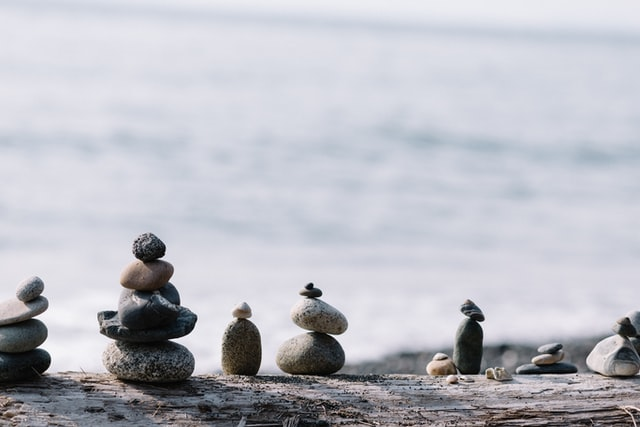
\includegraphics[width=.4\textwidth, align=c]{balance}
    &
      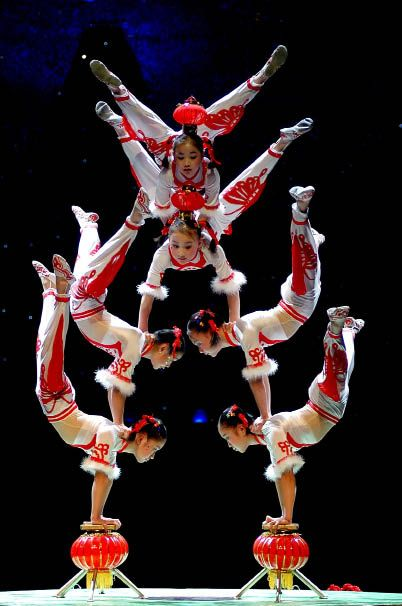
\includegraphics[height=.3\textheight, align=c]{circus}
    &
    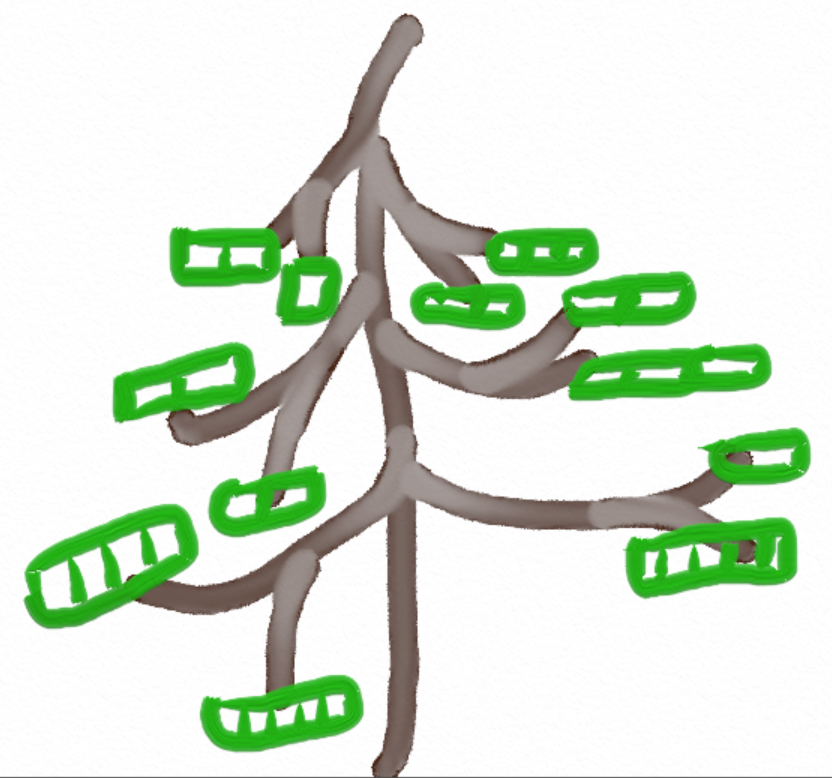
\includegraphics[width=.25\textwidth, align=c]{btree}
    \\
    \\
    (a) Balance, Photo by \href{https://unsplash.com/@patrickian4?utm_source=unsplash&utm_medium=referral&utm_content=creditCopyText}{Patrick Fore} on \href{https://unsplash.com/?utm_source=unsplash&utm_medium=referral&utm_content=creditCopyText}{Unsplash}
                                                                                                                                                                                                      & (b) Structure,
    & (c) B-Tree\\
&  \href{https://www.pinterest.co.uk/pin/29132728826423616/}{Chinese Circus} by \href{http://www.chinatoday.com.cn/}{China Today}
  \end{tabular}
  \caption{Positive and negative examples of abstraction.} 
  \label{fig:example}
\end{figure}

Figure \ref{fig:example} shows examples of abstracted art work. The figure (a) would be an acceptable submission for the topic of ``Balanced trees''. It represents balance and structure. The submission would be worthier if the sizes and quantities of the stones were in some particular order, or they were colored a particular way. The figure (b) could be a depiction of the course as it represents order, structure, organization, balance, effort, and ingenuity. All of these are traits that we encountered in this course. It would be a worthier submission if it showed various other simultaneous configurations, thus denoting that we encountered these traits in various forms throughout this course.

The figure (c) would be an unacceptable submission for B-Tree. It is a literal depiction and leaves a lot of room for artistic improvement.

\section*{Accompaniment}

Do the above examples lend themselves only to the explanations given above? Definitely not. It is art, it can have many different interpretations, none less valid than the other! For your art work, you have to provide an accompanying explanation of what it depicts (the subject) and how (the depiction). The subject must be appropriate to the content of the course and the depiction must be readily understandable once explained. The depiction must not be vulgar, offensive, or disrespectful. 

\section*{Abstraction and Aesthetics}

Your submitted art work should be an abstract depiction of your chosen subject. It should also be aesthetically pleasing and tasteful. It should stand alone as a work of art, worthy of appreciation by someone who does not know about data structures, and invoking a pleasant nod of understanding by someone who does or has read your accompaniment. You should feel proud to frame and hang it on your drawing room wall, so that you can feel smug about it when your guests ask you how much you got it for and from which artist. Proceeds to Habib University ensuing from the successful sale of your art work is the subject of a separate discussion.

\section*{Submission}

Your art work may be in any digital format of your choosing: an image, an animation, video, audio, a website, a program, as long as it meets the requirements defined here and in the accompanying rubric. Any visual content must be at least \href{https://dsplay.tv/site/en/suporte/qual-a-diferenca-entre-resolucoes-hd-full-hd-ultra-hd-2k-4k-8k-10k/}{full HD resolution}. There must be an accompaniment containing an explanation of the subject and the depiction.

The submission must be an original work of art. Readily available photographs are provided as examples above for illustrative purposes only. Your submitted work may be hand drawn, digitally drawn, photographed, a collage, programmatically generated, or any mixture of these. Any significant effort spent in generating the work must be explained in the accompaniment, along with due acknowledgment of all used sources. Works of performed art are sadly not eligible in this offering.

\bigskip

\hrulefill \textit{Good Luck!} \hrulefill

\end{document}

%%% Local Variables:
%%% mode: latex
%%% TeX-master: t
%%% End:
